\documentclass[runningheads]{llncs}

\usepackage[utf8]{inputenc}
\usepackage{graphicx}
% Used for displaying a sample figure. If possible, figure files should
% be included in EPS format.
%
% If you use the hyperref package, please uncomment the following line
% to display URLs in blue roman font according to Springer's eBook style:
% \renewcommand\UrlFont{\color{blue}\rmfamily}

\begin{document}
%
\title{A greedy approach for the recomputation of the cluster centres in the FPAC Algorithm}


\author{Ivan Feliciano\inst{1} \and
Edgar Hernandez-Gonzalez\inst{2}}
%
\authorrunning{I. Feliciano et al.}
% First names are abbreviated in the running head.
% If there are more than two authors, 'et al.' is used.
%
\institute{National Institute of Astrophysics, Optics and Electronics
\email{ivan.felavel@gmail.com}\\
\and
National Institute of Astrophysics, Optics and Electronics\\
\email{edgarmoy.28@gmail.com}}
\maketitle              % typeset the header of the contribution
\begin{abstract}
En este trabajo presentamos una modificación al algoritmo K-means usando una heurística que permite hacer el recalculo de centroides de una manera diferente al k-means tradicional. El procedimiento se basa en…primero, después, por ultimo.

\keywords{First keyword  \and Second keyword \and Another keyword.}
\end{abstract}
%
%
%
\section{Introduction}
\subsection{A Subsection Sample}
Actualmente el numero de documentos en la web aumenta rápidamente, por tal motivo se necesitan algoritmos capaces de agrupar automáticamente grandes cantidades de datos.
K-means es un algoritmo de agrupamiento, su objetivo es particionar un conjunto de datos en k grupos basándose en sus características. El agrupamiento se realiza minimizando la suma de distancias entre cada objeto y el centroide de su grupo.
El algoritmo consta de tres pasos:
1.	Inicialización: una vez escogido el número de grupos, k, se establecen k centroides en el espacio de los datos, por ejemplo, escogiéndolos aleatoriamente.
2.	Asignación objetos a los centroides: cada objeto de los datos es asignado a su centroide más cercano.
3.	Actualización centroides: se actualiza la posición del centroide de cada grupo tomando como nuevo centroide la posición del promedio de los objetos pertenecientes a dicho grupo.
Se repiten los pasos 2 y 3 hasta que los centroides no se mueven, o se mueven por debajo de una distancia umbral en cada paso.
A pesar de que el algoritmo K-means es muy popular no es escalable para datos de gran tamaño y dimensión.
El principal cuello de botella de K-means es asignar cada vector no centroide a un grupo.


\subsubsection{Sample Heading (Third Level)} Only two levels of
headings should be numbered. Lower level headings remain unnumbered;
they are formatted as run-in headings.

\paragraph{Sample Heading (Fourth Level)}
The contribution should contain no more than four levels of
headings. Table~\ref{tab1} gives a summary of all heading levels.

\begin{table}
\caption{Table captions should be placed above the
tables.}\label{tab1}
\begin{tabular}{|l|l|l|}
\hline
Heading level &  Example & Font size and style\\
\hline
Title (centered) &  {\Large\bfseries Lecture Notes} & 14 point, bold\\
1st-level heading &  {\large\bfseries 1 Introduction} & 12 point, bold\\
2nd-level heading & {\bfseries 2.1 Printing Area} & 10 point, bold\\
3rd-level heading & {\bfseries Run-in Heading in Bold.} Text follows & 10 point, bold\\
4th-level heading & {\itshape Lowest Level Heading.} Text follows & 10 point, italic\\
\hline
\end{tabular}
\end{table}


\noindent Displayed equations are centered and set on a separate
line.
\begin{equation}
x + y = z
\end{equation}
Please try to avoid rasterized images for line-art diagrams and
schemas. Whenever possible, use vector graphics instead (see
Fig.~\ref{fig1}).

\begin{figure}
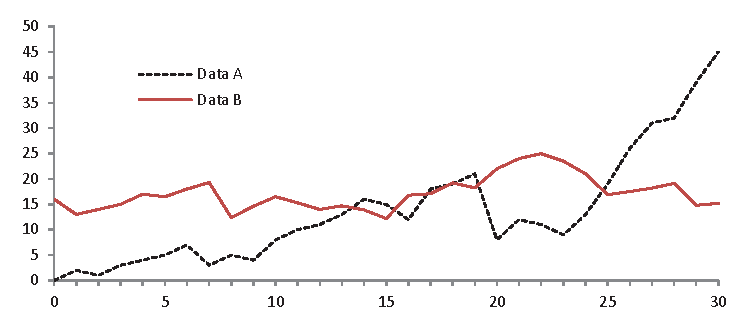
\includegraphics[width=\textwidth]{fig1.eps}
\caption{A figure caption is always placed below the illustration.
Please note that short captions are centered, while long ones are
justified by the macro package automatically.} \label{fig1}
\end{figure}

\begin{theorem}
This is a sample theorem. The run-in heading is set in bold, while
the following text appears in italics. Definitions, lemmas,
propositions, and corollaries are styled the same way.
\end{theorem}
%
% the environments 'definition', 'lemma', 'proposition', 'corollary',
% 'remark', and 'example' are defined in the LLNCS documentclass as well.
%
\begin{proof}
Proofs, examples, and remarks have the initial word in italics,
while the following text appears in normal font.
\end{proof}
For citations of references, we prefer the use of square brackets
and consecutive numbers. Citations using labels or the author/year
convention are also acceptable. The following bibliography provides
a sample reference list with entries for journal
articles~\cite{ref_article1}, an LNCS chapter~\cite{ref_lncs1}, a
book~\cite{ref_book1}, proceedings without editors~\cite{ref_proc1},
and a homepage~\cite{ref_url1}. Multiple citations are grouped
\cite{ref_article1,ref_lncs1,ref_book1},
\cite{ref_article1,ref_book1,ref_proc1,ref_url1}.
\section{Related Work}
Se han hecho varias aportaciones para mejorar el algoritmo k-means.
[la del articulo] desarrollo un algoritmo de partición rápida basado en una heurística de los vecinos mas cercanos. Dado un conjunto de centroides, evitar el calculo de distancia por pares entre vectores para obtener una partición de la colección, en su lugar se ocupó una asignación basada en el vecino mas cercano de cada centro, para esto se utilizo una lista invertida de vectores dispersos.
También se evito el costoso calculo del centroide verdadero de cada grupo, se propuso una heurística para elegir el centroide de manera eficiente.
En [9] los autores utilizan la heurística más lejana primero que consiste en seleccionar los centroides iniciales y evitar los cálculos de distancia redundante desde los no centroides a los centros.
En [12, 19 y 20] se utilizaron estructuras de datos de partición de espacio como kd-trees. Esto aumenta la eficacia de k-means, pero solo para pocas dimensiones
En [23] reasignaciones de clúster ocurren frecuentemente para puntos que no están cerca de los centroides. Identifica estos puntos al agrupar puntos vecinos usando múltiples arboles de partición.
En [2 y 18] se utiliza una heurística la cual elije aleatoriamente el primer centroide y utiliza una distribución de probabilidad.
En [4] se utilizo k-means escalable en el cual cada centroide se ve como una consulta para recuperar una lista de documentos que luego se asignan a ese grupo sin cálculo de distancia.
[2] k-means ++.

\section{Proposed Solution}

\section{Experiments}

\section{Results}

\section{Conclusions and future work}

%
% ---- Bibliography ----
%
% BibTeX users should specify bibliography style 'splncs04'.
% References will then be sorted and formatted in the correct style.
%
% \bibliographystyle{splncs04}
% \bibliography{mybibliography}
%
\begin{thebibliography}{8}
\bibitem{ref_article1}
Author, F.: Article title. Journal \textbf{2}(5), 99--110 (2016)

\bibitem{ref_lncs1}
Author, F., Author, S.: Title of a proceedings paper. In: Editor,
F., Editor, S. (eds.) CONFERENCE 2016, LNCS, vol. 9999, pp. 1--13.
Springer, Heidelberg (2016). \doi{10.10007/1234567890}

\bibitem{ref_book1}
Author, F., Author, S., Author, T.: Book title. 2nd edn. Publisher,
Location (1999)

\bibitem{ref_proc1}
Author, A.-B.: Contribution title. In: 9th International Proceedings
on Proceedings, pp. 1--2. Publisher, Location (2010)

\bibitem{ref_url1}
LNCS Homepage, \url{http://www.springer.com/lncs}. Last accessed 4
Oct 2017
\end{thebibliography}
\end{document}
